%%
\subsection{Differenzieren}
Berechnung der Steigung der Funktion. ($\frac{dy}{dx}$)

\begin{center}
	\captionsetup{type=figure}
	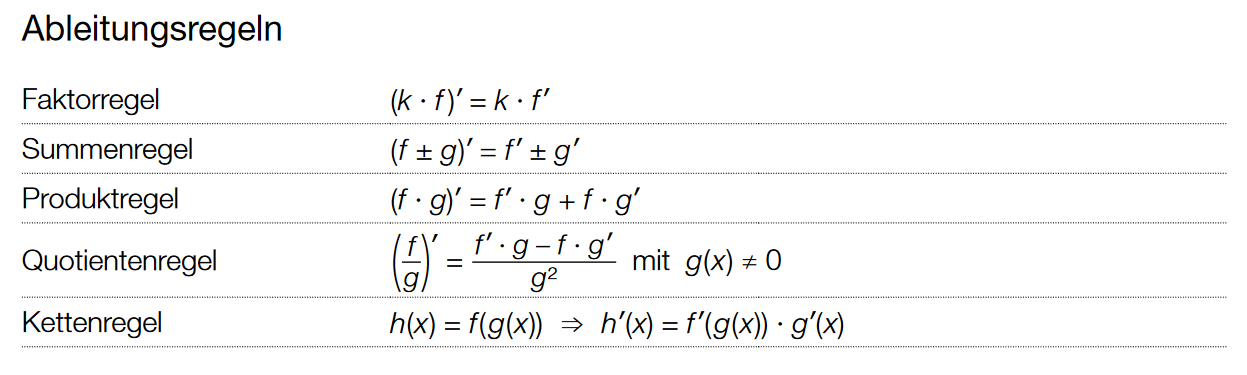
\includegraphics[width=0.9\linewidth]{pictures/Ableitungsregeln_Formelsammlung_Matura}
	\caption{Formelsammlung~\cite[S. 13]{Formelsammlung_BHS}}
	\label{fig:ableitungsregeln}
\end{center}



%%
\subsection{Integrieren}
Berechnung der Fläche zwischen der Funktion und der X-Achse. ($dx \cdot dy$)
\begin{enumerate}
	\item Man bestimme eine Stammfunktion $F(x)$ zum Integranden $f(x)$
	\item Mit dieser Stammfunktion berechnet man die Differnenz $F(b)-F(a)$
\end{enumerate}
\[\int\limits_a^b f(x) dx = \left . \left[F(x)\right] \right | _a^b = F(b)-F(a)\]

\textbf{unbestimmtes Integral:}
Das unbestimmte Integral gibt zu einer Funktion die Menge aller Stammfunktionen an.

%
\subsubsection{Grundintegrale}

\begin{center}
	\captionsetup{type=figure}
	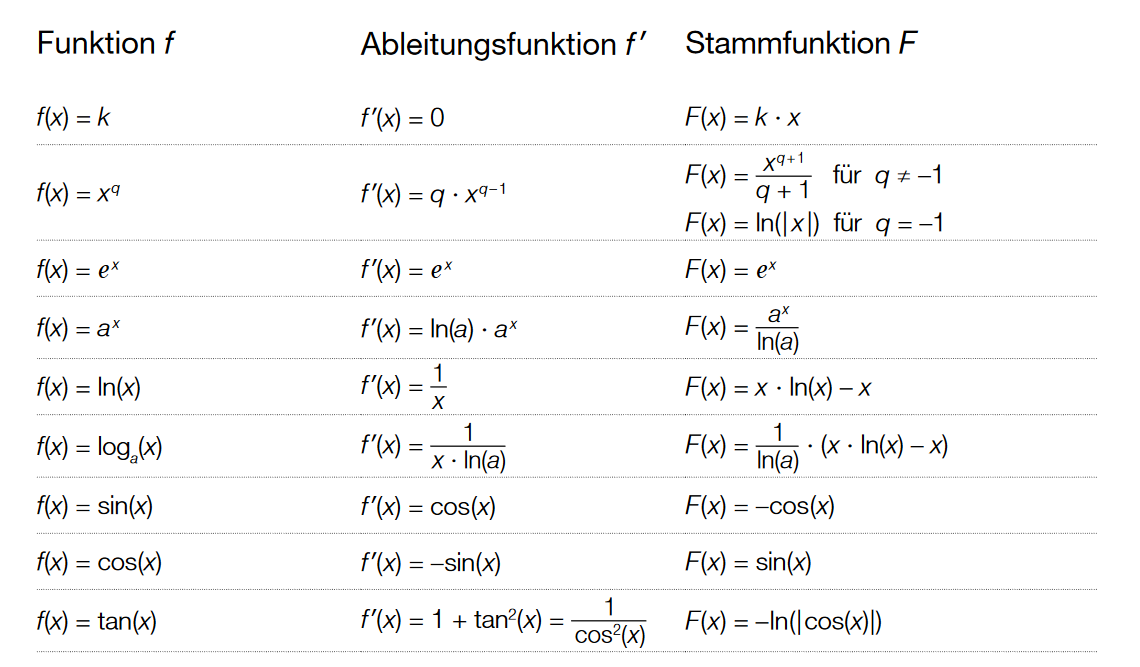
\includegraphics[width=0.9\linewidth]{pictures/Grundintegrale_Formelsammlung_BHS}
	\caption{Grundintegrale \cite[S. 13]{Formelsammlung_BHS}}
	\label{fig:grundintegrale}
\end{center}

%%
\subsubsection{Substituieren}
Bei Funktionen in Funktionen immer die innere Funktion substituieren.
Substitution wird gemacht, damit man die x wegkürzen kann. 
Wenn man eine substituierte Funktion integriert, müssen alle x weg sein! Integreieren nach u ist mit x in der Gleichung \textbf{nicht möglich}!!!\\
\[\int f\left[g(x)\right] dx = \int f(u) \frac{du}{g'(x)}\]

\subsubsection{Partielle Integration:}
\[\int u(x)\cdot v'(x)dx = u(x)\cdot v(x)-\int u(x)'\cdot v(x)dx\]

\subsubsection{Phönix Integral:}
$f(x)= \int g(x)h(x)dx$\\

Wenn weder $g(x)$ noch $h(x)$ beim Ableiten einfacher wird, sondern gleich bleibt oder sich wiederholt (Bsp.: $e^x, sin(x), cod(x)...$) wird solange partiell integriert, bis im Integral-Teil vom partiellen Integrieren die Ausgangsfunktion steht. Die beiden gleichen Integrale werden auf eine Seite gebracht und umgeformt bis $\int g(x)h(x)dx = ... $ dasteht.


%%
\subsection{Integrieren über den Betrag}
Beim Integrieren über einen Betrag muss die Funktion an jedem Nulldurchgang (falls vorhanden) aufgeteilt und integriert. Die negativen Stellen müssen in die Summe negativ eingehen.
Bsp.: $\int\limits_{0}^{e}|ln(x)| = |x*(ln(x)-1)|\big|_{0}^{e} = -x*(ln(x)-1)\big|_{0}^{1} + x*(ln(x)-1)\big|_{1}^{e}$ 
$\alpha$

%%%%
\subsection{Uneigentliche Integrale}
Ein Integral existiert, jedoch sind die Integrationsgrenzen nicht beschränkt.\\
\textbf{Fall 1:} Eine Grenze des Integrals ist $\infty$.
\[\int\limits_a^{\infty}f(x)dx = \lim \limits_{\lambda \to \infty}\int\limits_a^{\lambda}f(x)dx\]

\textbf{Fall 2:}
Eine Polstelle von f(x) liegt im zu integrierenden Bereich. Ist der Grenzwert des Integrals für $\lambda \to 0$ vorhanden, wird das uneigentliche Integral \textbf{konvergent} genannt, andernfalls heißt es \textbf{divergent}.\\
\textbf{Bsp.:} b ist Polstelle von f(x)\\
\[\int\limits_a^b f(x)dx=\lim\limits_{\lambda \to 0}\int\limits_a^{b-\lambda}f(x)dx\]
\textbf{Bsp.:} $c$ ist Polstelle von $f(x)$ mit $a<c<b$
\[\int\limits_a^b f(x) dx = \lim\limits_{\lambda \to 0}\int\limits_a^{c-\lambda}f(x)dx + \lim\limits_{\mu \to 0}\int\limits_a^{c-\mu}f(x)dx\]


%%%%
\subsection{Kurvenintegrale:}
Beim klassischen eindimensionalen Riemann- Integral integriert man über ein Intervall $[a,b]$ der reellen Achse.\\
Beim Kurvenintegral werden die integrationsbereiche als Kurven $C$ im $\mathbb{R}^n$ betrachtet.\\
\textbf{Kurvenintegral 1. Art:} Eine \textbf{reellwertige} Funktion $f:\mathbb{R}^n \ to \mathbb{R}$ wird über eine Kurve C integriert.\\
Es wird ein skalares Feld über eine Kurve integriert. Es kann zur berechnung der Länge einer Kurve sowie zur Berechnung linienhafter Ladungs/Masseverteilungen dienen.\\
\textbf{Kurvenintegral 2. Art (Arbeitsintegral):} Ein \textbf{Vektorfeld} wird über eine Kurve $C$ integriert. Dient zur Berechnung der nötigen Arbeit, um eine Masse/Ladung in einem Kraftfeld längs einer Kurve zu bewegen.\\

\textbf{Bogenelement:} $|\gamma'(t)dt|$\\

\subsubsection{Kurvenintegral 1. Art}
Für eine stückweise stetige Funktion $f:\mathbb{R}^n \to \mathbb{R}$ ist das Kurvenintegral von $f$ längs $\vec{\gamma}$: 
$$J=\int\limits_{\vec{\gamma}} fds = \int\limits_{t_a}^{t_e}f(\vec{\gamma} (t))\cdot |\dot{\gamma}(t)|dt$$

\textbf{Bsp.:} Bogenlänge $s(t)$ des Kurvenstücks $[t_a,t_e]$ der Kurve $C$:
\[s(t)=\int\limits_{t_a}^{t_e}\dot{\vec{\gamma}}(t)|dt= \int\limits_{t_a}^{t_e}\sqrt{\dot{x}_1^2(t) + \dot{x}_2^2(t) + \dot{x}_n^2(t)}dt\]

\textbf{Algorythmus zum Berechnen eines Kurvenintegrales 1. Art:}
\begin{itemize}
	\item Parametrisierung der Kurve $\vec{\gamma}(t)$
	\item Berechnung der Funktionswerte $f(\vec{\gamma}(t))$ der Belegungsfunktion
	\item Berechnung von $|\dot{\vec{\gamma}}(t)|$
	\item Berechnung des Kurvenintegrals
\end{itemize}
$$\int\limits_{\vec{\gamma}} fds = \int\limits_{t_a}^{t_e}f(\vec{\gamma} (t))\cdot |\dot{\vec{\gamma}}(t)|dt$$

\subsubsection{Kurvenintegral 2. Art}
\begin{itemize}
	\item Parametrisierung der Kurve $\vec{\gamma}:[t_a,t_e]\to \mathbb{R}^n$
	\item Berechnung der Werte $k(\vec{\gamma}(t))$ in den Kurvenpunkten
	\item Berechnung des Tangentenvektors $|\dot{\vec{\gamma}}(t)|$
	\item Berechnung des Kurvenintegrals
\end{itemize}
$$\int\limits_{\vec{\gamma}} kds = \int\limits_{t_a}^{t_e}k(\vec{\gamma} (t))\cdot \dot{\vec{\gamma}}(t)dt$$

\subsection{Gebietsintegrale / Doppelintegrale}
Skript 2022x11x29 Seite 9\\

Keine Flächenberechnung!! Es wird das Volumen, welches vom Skalarfeld und der $x/y$ Ebene im Gebiet $G$ eingeschlossen wird, berechnet.\\

$f(x,y)$... Skalarfeld, $f_{1/2}(x)$... untere/obere \grqq Beschänkungsfunktion\grqq{}, $G$... Gebiet welches von $f_{1/2}(x)$ eingeschlossen wird.

\[\int \int\limits_{(G)}f(x,y) dG = \int\limits_{a_1}^{a_2} \left( \int\limits_{f_1(x)}^{f_2(x)}f(x,y)dy\right)dx\]

\captionsetup{type=figure}
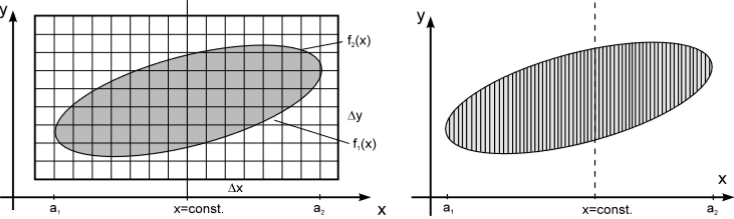
\includegraphics[width= \textwidth]{../pictures/Gebietsintegrale.png}
\caption{Gebietsintegrale}\label{fig:Gebietsintegrale}

\begin{itemize}
	\item es ist egal, ob zuerst nach $x$ oder $y$ integriert wird (wählen was einfacher ist).
	\item Bei Integration nach y: $y(x)$ für die Obere- und Untere- Begrenzungsfunktion berechnen.
	\item nach y integrieren. Mit dem somit berechneten Integral wird die \grqq Strichlänge \grqq{} (eigentlich die Fläche zwischen der $x/y$ Ebene und dem Strich) abhängig von x berechnet.
	\item Von $a_1$ bis $a_2$ über $x$ integrieren. (wird zuerst nach $x$ integriert, $x$ und $y$ jeweils vertauschen)
\end{itemize}